\begin{frame}[plain]
    \hspace{2cm}
    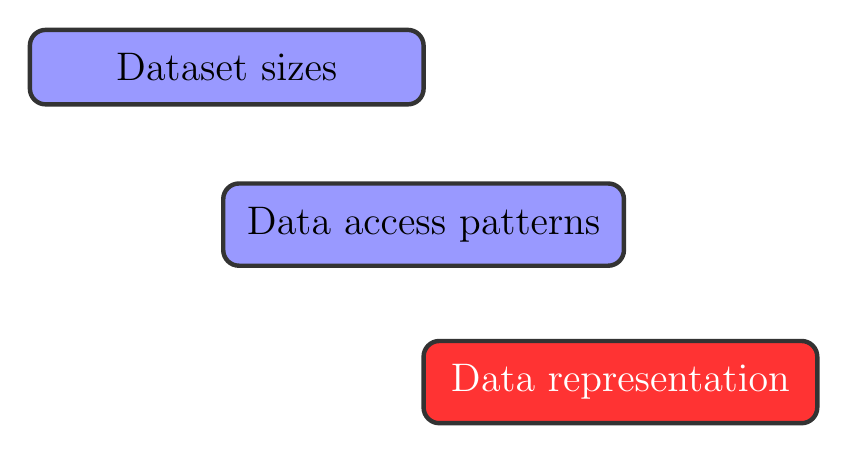
\begin{tikzpicture}[
        norm/.style={draw=black!80,rectangle,rounded corners=2mm,inner sep=3mm,fill=blue!40,ultra thick,minimum width=5cm},
        lit/.style={draw=black!80,rectangle,rounded corners=2mm,inner sep=3mm,fill=red!80,ultra thick,minimum width=5cm}
      ]
      \node[norm] at (0,0) {{\Large Dataset sizes}};
      \node[norm] at (2.5,-2) {{\Large Data access patterns}};
      \node[lit] at (5,-4) {{\Large \textcolor{white}{Data representation}}};
    \end{tikzpicture}
\end{frame}

\begin{frame}[plain]
  \begin{block}{Science Modules}
    \vspace{1cm}
    \hspace{2cm}
    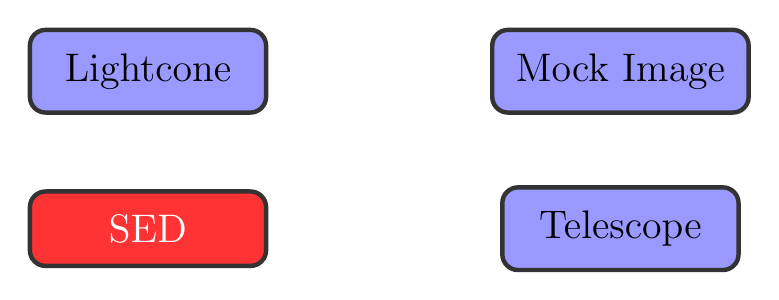
\begin{tikzpicture}[
        norm/.style={draw=black!80,rectangle,rounded corners=2mm,inner sep=3mm,fill=blue!40,ultra thick,minimum width=3cm},
        lit/.style={draw=black!80,rectangle,rounded corners=2mm,inner sep=3mm,fill=red!80,ultra thick,minimum width=3cm}
      ]
      \node[norm] at (0,0) {{\Large Lightcone}};
      \node[lit] at (0,-2) {{\Large \textcolor{white}{SED}}};
      \node[norm] at (6,0) {{\Large Mock Image}};
      \node[norm] at (6,-2) {{\Large Telescope}};
    \end{tikzpicture}
    \vspace{1cm}
  \end{block}
\end{frame}

\begin{frame}[plain]
 \begin{tikzpicture}[
     gal/.style={circle,draw},
     level 2/.style={sibling distance=10mm}
   ]
   \path[use as bounding box] (-2,-1.5) rectangle (8,6.5);
   % Merger trees.
   \node[gal] at (0,0) {I} [grow'=up]
     child {node {} edge from parent[dashed]};
   \node[gal] at (3,0) {A} [grow'=up]
     child {node[gal] {B}
       child {node[gal] {F}
         child {node[gal] {G}}
         child {node[gal] {H}}
       }
     }
     child {node[gal] {C}
       child {node[gal] {D}}
       child {node[gal] {E}}
     };
   \node[gal] at (6,0) {J} [grow'=up]
     child {node {} edge from parent[dashed]};
 \end{tikzpicture}
\end{frame}

\begin{frame}[plain]
 \begin{tikzpicture}[
     gal/.style={circle,draw},
     level 2/.style={sibling distance=10mm}
   ]
   \path[use as bounding box] (-2,-1.5) rectangle (8,6.5);
   % Merger trees.
   \node[gal] at (0,0) {I} [grow'=up]
     child {node {} edge from parent[dashed]};
   \node[gal] at (3,0) {A} [grow'=up]
     child {node[gal] {B}
       child {node[gal] {F}
         child {node[gal] {G}}
         child {node[gal] {H}}
       }
     }
     child {node[gal] {C}
       child {node[gal] {D}}
       child {node[gal] {E}}
     };
   \node[gal] at (6,0) {J} [grow'=up]
     child {node {} edge from parent[dashed]};
   % Pointers.
   \draw[-triangle 90] (5,5.5) node[anchor=west] {earliest galaxies} .. controls(2.25,5.5)and(2.25,5.5) .. (2.25,5);
 \end{tikzpicture}
\end{frame}

\begin{frame}[plain]
 \begin{tikzpicture}[
     gal/.style={circle,draw},
     level 2/.style={sibling distance=10mm}
   ]
   \path[use as bounding box] (-2,-1.5) rectangle (8,6.5);
   % Merger trees.
   \node[gal] at (0,0) {I} [grow'=up]
     child {node {} edge from parent[dashed]};
   \node[gal] at (3,0) {A} [grow'=up]
     child {node[gal] {B}
       child {node[gal] {F}
         child {node[gal] {G}}
         child {node[gal] {H}}
       }
     }
     child {node[gal] {C}
       child {node[gal] {D}}
       child {node[gal] {E}}
     };
   \node[gal] at (6,0) {J} [grow'=up]
     child {node {} edge from parent[dashed]};
   % Pointers.
   \draw[-triangle 90] (5,5.5) node[anchor=west] {earliest galaxies} .. controls(2.25,5.5)and(2.25,5.5) .. (2.25,5);
   \draw[-triangle 90] (1,4) node[anchor=east] {galaxies merge} -- (2,3.25);
   \draw[-triangle 90] (6,3) node[anchor=west] {galaxies merge} -- (4,1.75);
 \end{tikzpicture}
\end{frame}

\begin{frame}[plain]
 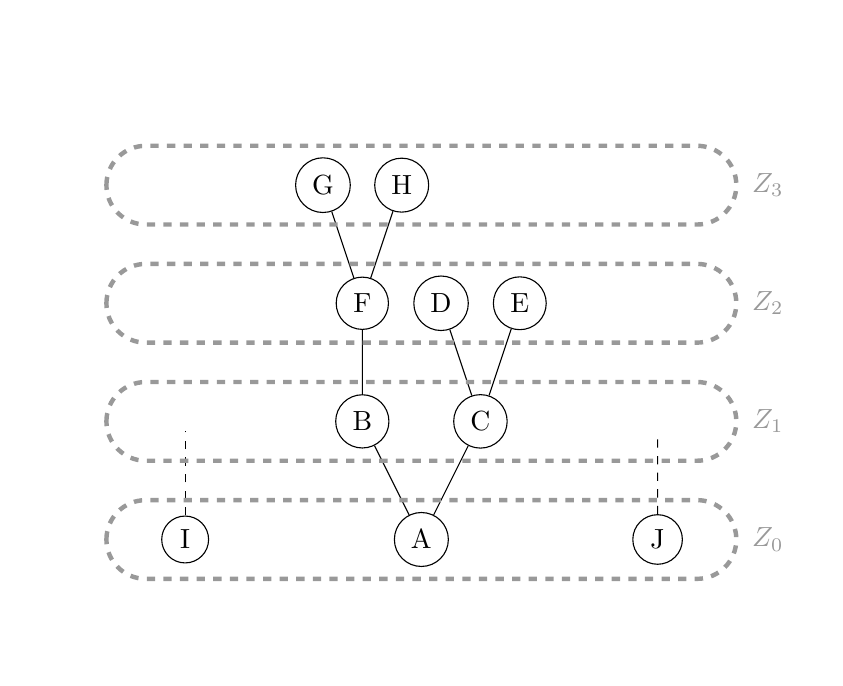
\begin{tikzpicture}[
     gal/.style={circle,draw},
     level 2/.style={sibling distance=10mm}
   ]
   \path[use as bounding box] (-2,-1.5) rectangle (8,6.5);
   % Merger trees.
   \node[gal] at (0,0) {I} [grow'=up]
     child {node {} edge from parent[dashed]};
   \node[gal] at (3,0) {A} [grow'=up]
     child {node[gal] {B}
       child {node[gal] {F}
         child {node[gal] {G}}
         child {node[gal] {H}}
       }
     }
     child {node[gal] {C}
       child {node[gal] {D}}
       child {node[gal] {E}}
     };
   \node[gal] at (6,0) {J} [grow'=up]
     child {node {} edge from parent[dashed]};
   % Snapshots.
   \draw[ultra thick,black!40,dashed,rounded corners=5mm] (-1,-0.5) rectangle (7,0.5) node[black!40] at (7.4,0) {$Z_0$};
   \draw[ultra thick,black!40,dashed,rounded corners=5mm] (-1,1) rectangle (7,2) node[black!40] at (7.4,1.5) {$Z_1$};
   \draw[ultra thick,black!40,dashed,rounded corners=5mm] (-1,2.5) rectangle (7,3.5) node[black!40] at (7.4,3) {$Z_2$};
   \draw[ultra thick,black!40,dashed,rounded corners=5mm] (-1,4) rectangle (7,5) node[black!40] at (7.4,4.5) {$Z_3$};
 \end{tikzpicture}
\end{frame}

\begin{frame}[plain]
 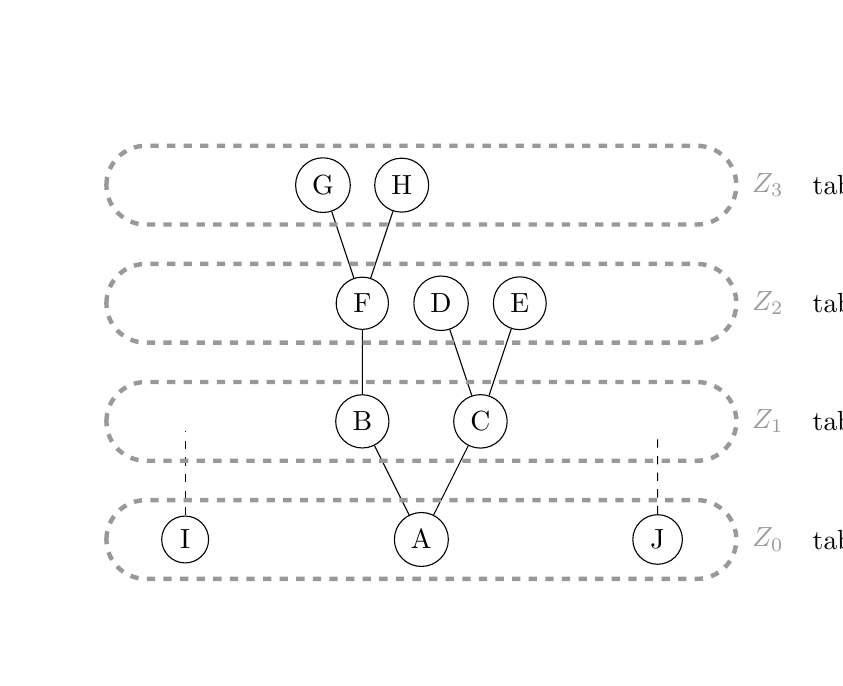
\begin{tikzpicture}[
     gal/.style={circle,draw},
     level 2/.style={sibling distance=10mm}
   ]
   \path[use as bounding box] (-2,-1.5) rectangle (8,6.5);
   % Merger trees.
   \node[gal] at (0,0) {I} [grow'=up]
     child {node {} edge from parent[dashed]};
   \node[gal] at (3,0) {A} [grow'=up]
     child {node[gal] {B}
       child {node[gal] {F}
         child {node[gal] {G}}
         child {node[gal] {H}}
       }
     }
     child {node[gal] {C}
       child {node[gal] {D}}
       child {node[gal] {E}}
     };
   \node[gal] at (6,0) {J} [grow'=up]
     child {node {} edge from parent[dashed]};
   % Snapshots.
   \draw[ultra thick,black!40,dashed,rounded corners=5mm] (-1,-0.5) rectangle (7,0.5) node[black!40] at (7.4,0) {$Z_0$} node[black] at (8.5,0) {table\_0};
   \draw[ultra thick,black!40,dashed,rounded corners=5mm] (-1,1) rectangle (7,2) node[black!40] at (7.4,1.5) {$Z_1$} node[black] at (8.5,1.5) {table\_1};
   \draw[ultra thick,black!40,dashed,rounded corners=5mm] (-1,2.5) rectangle (7,3.5) node[black!40] at (7.4,3) {$Z_2$} node[black] at (8.5,3) {table\_2};
   \draw[ultra thick,black!40,dashed,rounded corners=5mm] (-1,4) rectangle (7,5) node[black!40] at (7.4,4.5) {$Z_3$} node[black] at (8.5,4.5) {table\_3};
 \end{tikzpicture}
\end{frame}

\begin{frame}[plain]
 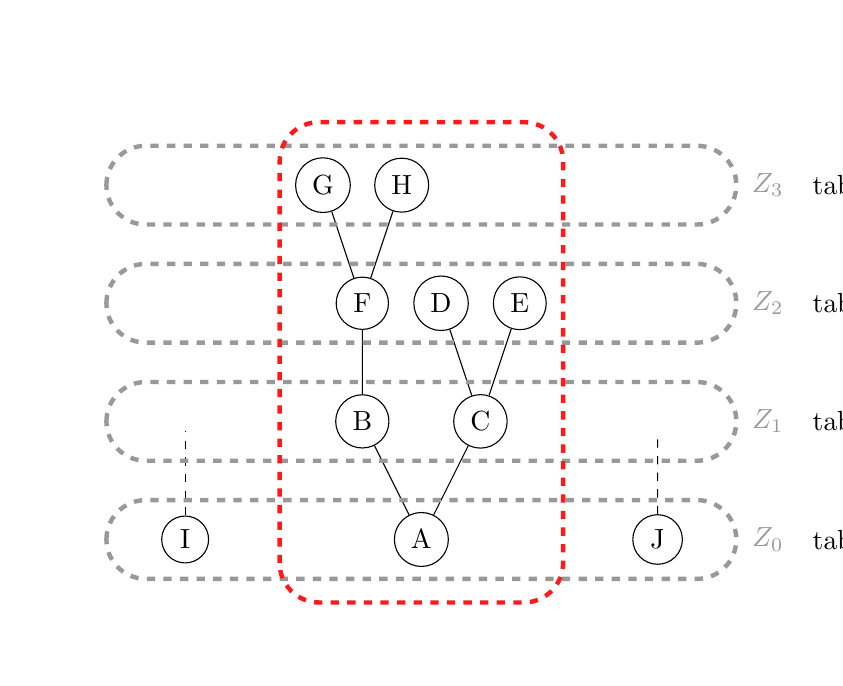
\begin{tikzpicture}[
     gal/.style={circle,draw},
     level 2/.style={sibling distance=10mm}
   ]
   \path[use as bounding box] (-2,-1.5) rectangle (8,6.5);
   % Merger trees.
   \node[gal] at (0,0) {I} [grow'=up]
     child {node {} edge from parent[dashed]};
   \node[gal] at (3,0) {A} [grow'=up]
     child {node[gal] {B}
       child {node[gal] {F}
         child {node[gal] {G}}
         child {node[gal] {H}}
       }
     }
     child {node[gal] {C}
       child {node[gal] {D}}
       child {node[gal] {E}}
     };
   \node[gal] at (6,0) {J} [grow'=up]
     child {node {} edge from parent[dashed]};
   % Snapshots.
   \draw[ultra thick,black!40,dashed,rounded corners=5mm] (-1,-0.5) rectangle (7,0.5) node[black!40] at (7.4,0) {$Z_0$} node[black] at (8.5,0) {table\_0};
   \draw[ultra thick,black!40,dashed,rounded corners=5mm] (-1,1) rectangle (7,2) node[black!40] at (7.4,1.5) {$Z_1$} node[black] at (8.5,1.5) {table\_1};
   \draw[ultra thick,black!40,dashed,rounded corners=5mm] (-1,2.5) rectangle (7,3.5) node[black!40] at (7.4,3) {$Z_2$} node[black] at (8.5,3) {table\_2};
   \draw[ultra thick,black!40,dashed,rounded corners=5mm] (-1,4) rectangle (7,5) node[black!40] at (7.4,4.5) {$Z_3$} node[black] at (8.5,4.5) {table\_3};
   % Forest.
   \draw[ultra thick,red!90,dashed,rounded corners=5mm] (1.2,-0.8) rectangle (4.8,5.3);
 \end{tikzpicture}
\end{frame}

\begin{frame}[plain]
 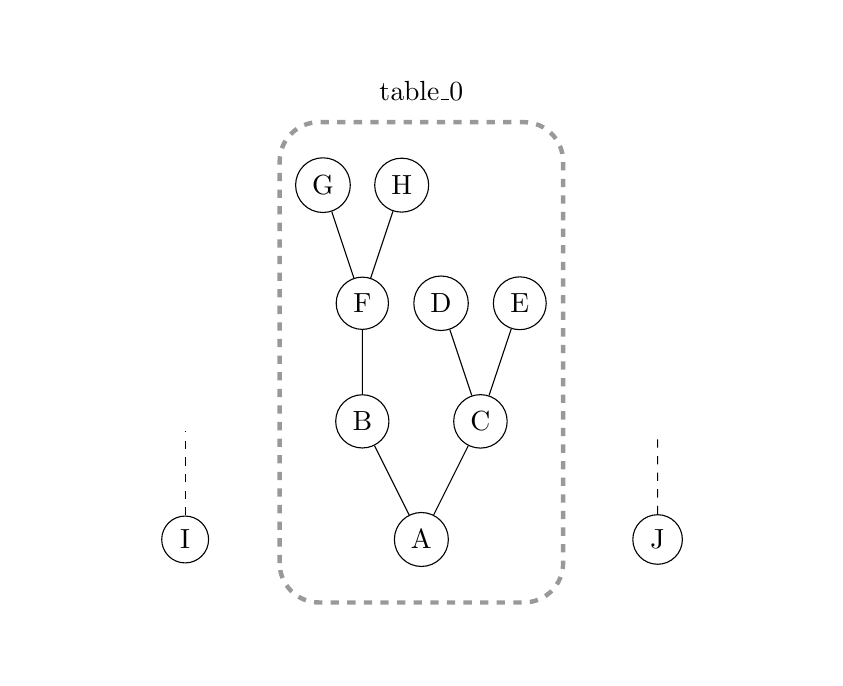
\begin{tikzpicture}[
     gal/.style={circle,draw},
     level 2/.style={sibling distance=10mm}
   ]
   \path[use as bounding box] (-2,-1.5) rectangle (8,6.5);
   % Merger trees.
   \node[gal] at (0,0) {I} [grow'=up]
     child {node {} edge from parent[dashed]};
   \node[gal] at (3,0) {A} [grow'=up]
     child {node[gal] {B}
       child {node[gal] {F}
         child {node[gal] {G}}
         child {node[gal] {H}}
       }
     }
     child {node[gal] {C}
       child {node[gal] {D}}
       child {node[gal] {E}}
     };
   \node[gal] at (6,0) {J} [grow'=up]
     child {node {} edge from parent[dashed]};
   % Forest.
   \draw[ultra thick,black!40,dashed,rounded corners=5mm] (1.2,-0.8) rectangle (4.8,5.3) node[black] at (3,5.7) {table\_0};
 \end{tikzpicture}
\end{frame}

%%
%% Rebinning.
%%

%% \begin{frame}[plain]
%%  \begin{tikzpicture}[
%%      gal/.style={circle,draw},
%%      main/.style={circle,draw,fill=red!80},
%%      lit/.style={circle,draw,fill=blue!40},
%%      level 2/.style={sibling distance=10mm}
%%    ]
%%    % Bounds.
%%    \path[use as bounding box] (-5,0) rectangle (5,6.5);
%%    % Text.
%%    \node at (-3.5,3) {Wrong timescale!};
%%    % Merger tree
%%    \node[gal] {A} [grow'=up]
%%      child {node[gal] {B}
%%        child {node[gal] {F}
%%          child {node[gal] {G}}
%%          child {node[gal] {H}}
%%        }
%%      }
%%      child {node[gal] {C}
%%        child {node[gal] {D}}
%%        child {node[gal] {E}}
%%      };
%%    % Snapshots.
%%    \draw (2.65,-0.05) -- (2.65,4.55);
%%    \foreach \y/\z in {-0.05/0, 1.55/1, 3.05/2, 4.55/3}
%%      \draw (2.6,\y) -- (2.7,\y) node[anchor=west] {$Z_\z$};
%%  \end{tikzpicture}
%% \end{frame}

%% \begin{frame}[plain]
%%  \begin{tikzpicture}[
%%      gal/.style={circle,draw},
%%      main/.style={circle,draw,fill=red!80},
%%      lit/.style={circle,draw,fill=blue!40},
%%      level 2/.style={sibling distance=10mm}
%%    ]
%%    % Bounds.
%%    \path[use as bounding box] (-5,0) rectangle (5,6.5);
%%    % Merger tree
%%    \node[main] {\textcolor{white}{A}} [grow'=up]
%%      child {node[lit] {B}
%%        child {node[lit] {F}
%%          child {node[lit] {G}}
%%          child {node[lit] {H}}
%%        }
%%      }
%%      child {node[lit] {C}
%%        child {node[lit] {D}}
%%        child {node[lit] {E}}
%%      };
%%    % Snapshots.
%%    \draw (2.65,-0.05) -- (2.65,4.55);
%%    \foreach \y/\z in {-0.05/0, 1.55/1, 3.05/2, 4.55/3}
%%      \draw (2.6,\y) -- (2.7,\y) node[anchor=west] {$Z_\z$};
%%    % Rebinning.
%%    \draw (4.05,-0.05) -- (4.05,6);
%%    \foreach \y/\z in {-0.05/0, 1/1, 3/2, 6/3}
%%      \draw (4,\y) -- (4.1,\y) node[anchor=west] {$\bar{Z}_\z$};
%%  \end{tikzpicture}
%% \end{frame}

%% \begin{frame}[plain]
%%  \begin{tikzpicture}[
%%      gal/.style={circle,draw},
%%      main/.style={circle,draw,fill=red!80},
%%      lit/.style={circle,draw,fill=blue!40},
%%      level 2/.style={sibling distance=10mm}
%%    ]
%%    % Bounds.
%%    \path[use as bounding box] (-5,0) rectangle (5,6.5);
%%    % Merger tree
%%    \node[gal] {A} [grow'=up]
%%      child {node[main] {\textcolor{white}{B}}
%%        child {node[lit] {F}
%%          child {node[lit] {G}}
%%          child {node[lit] {H}}
%%        }
%%      }
%%      child {node[gal] {C}
%%        child {node[gal] {D}}
%%        child {node[gal] {E}}
%%      };
%%    % Snapshots.
%%    \draw (2.65,-0.05) -- (2.65,4.55);
%%    \foreach \y/\z in {-0.05/0, 1.55/1, 3.05/2, 4.55/3}
%%      \draw (2.6,\y) -- (2.7,\y) node[anchor=west] {$Z_\z$};
%%    % Rebinning.
%%    \draw (4.05,1.55) -- (4.05,4.6);
%%    \draw[dashed] (4.05,4.6) -- (4.05,6);
%%    \foreach \y/\z in {1.55/0, 2.6/1, 4.6/2}
%%      \draw (4,\y) -- (4.1,\y) node[anchor=west] {$\bar{Z}_\z$};
%%  \end{tikzpicture}
%% \end{frame}
